%%%% ijcai17.tex

\typeout{IJCAI-17 Instructions for Authors}

% These are the instructions for authors for IJCAI-17.
% They are the same as the ones for IJCAI-11 with superficical wording
%   changes only.

\documentclass{article}
% The file ijcai17.sty is the style file for IJCAI-17 (same as ijcai07.sty).
\usepackage{ijcai17}
\usepackage{graphicx}
\usepackage{subfigure}
\usepackage{amsmath,amsfonts}
\usepackage{algorithm,algorithmic}
\renewcommand{\algorithmicrequire}{\textbf{Input:}}
\renewcommand{\algorithmicensure}{\textbf{Output:}}
% Use the postscript times font!
\usepackage{times}
\def \y {\mathbf{y}}
\def \x {\mathbf{x}}
\def \Y {\mathbf{Y}}
\def \X {\mathbf{X}}
\def \w {\mathbf{w}}
\def \v {\mathbf{v}}
\def \V {\mathbf{V}}
\def \Z {\mathbf{Z}}
\def \z {\mathbf{z}}
% the following package is optional:
%\usepackage{latexsym}

% Following comment is from ijcai97-submit.tex:
% The preparation of these files was supported by Schlumberger Palo Alto
% Research, AT\&T Bell Laboratories, and Morgan Kaufmann Publishers.
% Shirley Jowell, of Morgan Kaufmann Publishers, and Peter F.
% Patel-Schneider, of AT\&T Bell Laboratories collaborated on their
% preparation.

% These instructions can be modified and used in other conferences as long
% as credit to the authors and supporting agencies is retained, this notice
% is not changed, and further modification or reuse is not restricted.
% Neither Shirley Jowell nor Peter F. Patel-Schneider can be listed as
% contacts for providing assistance without their prior permission.

% To use for other conferences, change references to files and the
% conference appropriate and use other authors, contacts, publishers, and
% organizations.
% Also change the deadline and address for returning papers and the length and
% page charge instructions.
% Put where the files are available in the appropriate places.

\title{Locally Linear Factorization Machine}
\author{Anonymous Author(s) \\
Affiliation \\
email}

\begin{document}

\maketitle

\begin{abstract}

\end{abstract}

\section{Introduction}

\section{Related work}
\section{Locally Linear Factorization Machine Model}
Factorization machines (FMs) \cite{rendle2010factorization,rendle2012factorization} are a widely used method for efficiently using high-order feature interaction in classification and regression tasks even when the data is very high-dimensional. A standard $2$-order factorization machine model takes the form:
\begin{align}
f(\x) = \sum^p_{j=1}w_j x_j + \sum^p_{j=1}\sum^p_{j^\prime = j +1} x_j x_{j^\prime}\sum^k_{f=1}v_{j,f}v_{j^\prime,f},
\end{align}
where $p$ is the dimensionality of feature vector $\x \in \mathbb{R}^p$, $k \ll p$ is a hyper-parameter that denotes the dimensionality of latent factors, and $ w_j, v_{j,f}$ are the model parameters to be estimated, i.e., $\Theta=\{w_1,\dots,w_n,v_{1,1},\dots,v_{p,k}\}=\{\w \in \mathbb{R}^{p},\V \in \mathbb{R}^{p \times k}\}$. It is equivalent to the following simple equation:
\begin{align}
f(\x) = \w^\top\x+\sum^p_{j=1}\sum^p_{j^\prime=j+1}(\V\V^\top)_{jj^\prime}x_jx_{j^\prime},
\end{align}
The main advantage of FMs compared to the polynomial kernel in SVM \cite{vapnik2013nature} is the pairwise feature interaction weight matrix $\Z = \V\V^\top \in \mathbb{S}^{p \times p}$, where the number of parameters to estimate is reduced from $p^2$ to $kp$ by utilizing the factorized form. In addition, this factorization form helps to drop the prediction cost to linear runtime by utilizing
\begin{align}
f(\x) = \w^\top\x + \frac{1}{2}\left(\|\V^\top\x\|^2-\sum^k_{f=1}\|\v_f\circ\x\|^2\right),
\end{align}
where $\v_f\in\mathbb{R}^p$ is the $f^{th}$ column of $\V$ and $\circ$ denotes the element-wise product between two vectors by $\v_f \circ \x = [v_{f_1}x_1,\dots,v_{fp}x_p]^\top$. Thus, the computation cost is in $O(kp)$ instead of $O(p^2)$. Moreover, under sparsity condition, the prediction cost reduces to $O(kN_z(\x))$, where $N_z(\x)$ is the number of non-zero features in $\x$. Given a training set consisting of $n$ feature vectors $\X = [\x_1,\dots,\x_n]^\top \in \mathbb{R}^{n\times p}$ and corresponding targets $\Y = [y_1,\dots,y_n]^\top \in \mathbb{R}^n$, model parameters $\Theta$ can be learned by using the principle of empirical risk minimization and solving the following non-convex problem
\begin{align}
\min\limits_{\w \in \mathbb{R}^p,\V\in\mathbb{R}^{p\times k}} \frac{1}{n}\sum^n_{i=1}\ell(y_i,f(\x))+\frac{\beta_1}{2}\|\w\|^2+\frac{\beta_2}{2}\|\V\|^2_F,
\end{align}
where $\beta_1 >0,\beta_2>0$ are hyper-parameters that avoid overfitting and $\ell$ is a convex loss function incurred. For regression task, we can adopt the squared loss $\ell(y,\hat{y})=\frac{1}{2}(y-f(\x))^2$. This optimization problem can be efficiently solved by many off-the-shelf approaches, such as stochastic gradient descent or coordinate descent methods which has been implemented in the libfm library \cite{rendle2012factorization}. Both methods have a runtime complexity of $O(kN_z(\x))$ under sparsity.

Factorization Machines haven been found successful in many prediction tasks, including classification, regression and ranking, due to its capability to model the pairwise feature interaction under low-rank constraint. However, Factorization Machines only consider the second order information of the input feature which limits their capacity in non-linear problems. Specifically, taking classification task into consideration, not all problems are approximately linearly separable after quadratic mapping. In most cases, real data naturally groups into clusters and lies on nearly disjoint lower dimensional manifolds and thus the original Factorization Machines are inapplicable. Although they have the capability of modeling the pairwise feature interaction, Factorization Machines  fail to capture the underlying structures of complex data. One intuitive idea for addressing this limitation is to leverage the manifold geometric structure to learn a nonlinear function which can be effectively approximated by a linear function with an coding under appropriate localization conditions. In other words, we assume that in a sufficiently small region the decision boundary is approximately linear and each data point $\x$ can then be approximated with a linear combination of surrounding anchor points, which are usually called local codings scheme.

Specifically, let $\{\z_j\}_{i=1}^m$ denote the set of $m$ anchor points, any point $\x$ is then approximated by a linear combination of surrounding anchor points as $
\x \approx \sum^m_{i=1}\gamma_{\z_i}(\x)\z_i,$
where $\gamma_{\z_i}(\x)$ (to be later defined) is the local coordinates, depicting the degree of membership of $\x$ to the $i$th anchor point $\z_i$, constrained by $\sum^m_{i=1}\gamma_{\z_i}(\x)=1$.

To encode this local linearity, the model parameters $\Theta$ of the Factorization Machines should vary according to the location of the point $\x$ in the feature space as:
\begin{align}
f_{LLFM}(\x)
= \w(\x)^\top\x+\sum^p_{j=1}\sum^p_{j^\prime=j+1}(\V(\x)\V(\x)^\top)_{jj^\prime}x_jx_{j^\prime}.
\end{align}
According to \cite{yu2009nonlinear,ladicky2011locally}, for a local coding scheme defined by anchor points $\v$, we can approximate the weight function $\w(\x),\V(\x)$ using local coding as:
\begin{align}
\label{model}
&f_{LLFM}(\x) \nonumber\\
=&\sum^m_{i=1}\gamma_{\z_i}(\x)\w_{\z_i}^\top\x+\sum^m_{i=1}\gamma_{\z_i}(\x)\sum^p_{j=1}\sum^p_{j^\prime=j+1}(\V_{\z_i}\V_{\z_i}^\top)_{jj^\prime}x_jx_{j^\prime} \nonumber \\
=&\sum^m_{i=1}\gamma_{\z_i}(\x)\left(\w_{\z_i}^\top\x+\sum^p_{j=1}\sum^p_{j^\prime=j+1}(\V_{\z_i}\V_{\z_i}^\top)_{jj^\prime}x_jx_{j^\prime}\right),
\end{align}
where $\Theta_{LLFM}=\{\Theta_{\z_i}\}^m_{i=1}=\{\w_{\z_i},\V_{\z_i}\}^m_{i=1}$ are the model parameters corresponding to the anchor point $\z_i$. This transformation can be seen as a finite kernel transforming a $p$-dimensional problem into a $mp$-dimensional one. It can also be interpreted as defining a locally linear Factorization Machines as the weighted average of $m$ separate Factorization Machines
with respect to each anchor point, where the weights are determined by the local coordinates $\gamma_{\z}(\x)$.

To evaluate $f_{LLFM}(\x)$ for each data point $\x$, we need to calculate the corresponding local coordinates $\gamma_{\z}(\x)$, which further depend on the anchor points $\z$ being used and the local coding scheme. Note that the prediction function in Eq.(\ref{model}) depends on both the model parameters $\w, \V$, the anchor point variable $\z$ and the local coding scheme. This leads to a natural two-step approach taken by existing methods \cite{ladicky2011locally,yu2009nonlinear}, which first estimate the anchor points for each data by adopting K-means clustering and evaluate the local codes with a predefined scheme, which usually utilizes exponential decay scheme or inversely-proportional decay scheme, and then feed the anchor points and the local codes to the downstream supervised model training. This two-step learning procedure is inconsistent
with our objective and rather suboptimal as the prediction information is not used in discovering the anchor points and the local codes, which is clearly not an optimal local coding scheme for prediction task as the two methods are not tightly coupled to fully exploit their potential.
\section{Optimization method for Joint learning Locally Linear Factorization Machines}
In this section we first discuss assumptions, then formulate the optimal estimation problem. Finally, we present our optimization approach for joint learning Locally Linear Factorization Machines.

\section{Experiments}
In this section, to verify the effectiveness of our proposed Adaptive Locally Linear Factorization Machines algorithm, we will compare 3 different adaptive algorithm to the original Factorization Machines algorithm on real-world datasets.
\subsection{Experimental Setup}
\subsubsection{Datasets}
We conduct our experiments on 2 real-wrold datasets, including Banana and IJCNN. The statistics of the datasets after preprocesing are shown in Table 1.
\begin{table}
	\caption{Basic statistics of datasets}
	\begin{tabular}{l*{6}{c}r}
		\hline
		Dataset              & train & test & feature \\
		\hline
		Banana 		   	& 3533 & 1767 & 2  \\
		IJCNN     	& 4990 & 91701 & 22   \\
	\end{tabular}
\end{table}
\subsubsection{Evaluation Metrics}
To illustrate the recommendation prediction quality of different methods, we use RMSE metric to evaluate the overall error.
\subsubsection{Methods}
In our experiments, we compare our 3 different locally linear Factorization Machines to baseline method (FM).
\begin{itemize}
	\item \textbf{LLFM}:FM with several fixed anchor points which initialized by K-means.
	\begin{algorithm}[H]
		\caption{LLFM}
		\begin{algorithmic}[1]
			\REQUIRE Training data $S$, the number of anchor points $m$, the number of nearest neighbors k, regularization parameter $\lambda$, learning rate $\eta$, parameter in Gaussian kernel $\beta$.
			\ENSURE Model parameters $\Theta = (\boldsymbol W, \boldsymbol V)$ and anchor points.
			\STATE Initialize anchor points v by K-means;Initialize $\Theta$:$\boldsymbol W\leftarrow(0,...,0),\boldsymbol V\sim N(0,0.1)$
			\REPEAT
			\FOR{$(\boldsymbol{x},y) \in S$}
			\STATE Compute the local coordinates $\gamma_{\boldsymbol{z}}(\boldsymbol{x})$
			\STATE Compute $\hat{y}(\boldsymbol{x}|\Theta)$
			\STATE Update $\boldsymbol W$
			\STATE Update $\boldsymbol V$
			\ENDFOR
			\UNTIL stopping criterion is met;
		\end{algorithmic}
	\end{algorithm}
	\item \textbf{LLFMAAP}:LLFM with Adaptive Anchor Points, update anchor points during learning phase. The anchor points are also initialized by K-means.
	\begin{algorithm}[H]
		\caption{LLFMAAP}
		\begin{algorithmic}[1]
			\REQUIRE Training data $S$, the number of anchor points $m$, the number of nearest neighbors k, regularization parameter $\lambda$, learning rate $\eta$, parameter in Gaussian kernel $\beta$.
			\ENSURE Model parameters $\Theta = (\boldsymbol W, \boldsymbol V)$ and anchor points.
			\STATE Initialize anchor points v by K-means;Initialize $\Theta$:$\boldsymbol W\leftarrow(0,...,0),\boldsymbol V\sim N(0,0.1)$
			\REPEAT
			\FOR{$(\boldsymbol{x},y) \in S$}
			\STATE Compute the local coordinates $\gamma_{\boldsymbol{z}}(\boldsymbol{x})$
			\STATE Compute $\hat{y}(\boldsymbol{x}|\Theta)$
			\STATE Update $\boldsymbol W$
			\STATE Update $\boldsymbol V$
			\FOR{$j=1$ \TO $k$}
			\STATE Update the $j$th nearest anchor point of $\boldsymbol{x}$.
			\ENDFOR
			\ENDFOR
			\UNTIL stopping criterion is met;
		\end{algorithmic}
	\end{algorithm}
	\item \textbf{LLFMAAPK}:LLFMAAP with Adaptive KNN, choose the optimal number of nearest neighbors of KNN for each sample. Also using adaptive anchor points like the former algorithm.
	\begin{algorithm}[H]
		\caption{LLFMAAPK}
		\begin{algorithmic}[1]
			\REQUIRE Training data $S$, the number of anchor points $m$, regularization parameter $\lambda$, learning rate $\eta$, Lipschitz to noise ratio $L/C$.
			\ENSURE Model parameters $\Theta = (\boldsymbol W, \boldsymbol V)$ and anchor points.
			\STATE Initialize anchor points v by K-means;Initialize $\Theta$:$\boldsymbol W\leftarrow(0,...,0),\boldsymbol V\sim N(0,0.1)$
			\REPEAT
			\FOR{$(\boldsymbol{x},y) \in S$}
			\STATE Compute the local coordinates $\gamma_{\boldsymbol{z}}(\boldsymbol{x})$ and the number of nearest neighbor $k_{\boldsymbol{z}}(\boldsymbol{x})$
			\STATE Compute $\hat{y}(\boldsymbol{x}|\Theta)$
			\STATE Update $\boldsymbol W$
			\STATE Update $\boldsymbol V$
			\FOR{$j=1$ \TO $k_{\boldsymbol{z}}(\boldsymbol{x})$}
			\STATE Update the jth nearest anchor point of $\boldsymbol{x}$.
			\ENDFOR
			\ENDFOR
			\UNTIL stopping criterion is met;
		\end{algorithmic}
	\end{algorithm}
\end{itemize}

\subsubsection{Hyper-parameter Settings}
We apply 5-fold cross validation to find the hyper-parameters for the four different algorithm independently. For parameter settings, we adopt the same parameter tuning schemes for all the compared algorithm to enable fair comparisons. We perform grid search to choose the best parameters for each algorithm on the training set.
\begin{itemize}
	\item \textbf{Learning rate} $\eta$: We do grid search in $\left\{0.001,0.005,0.01,0.05,0.1\right\}$.
	\item \textbf{Latent dimension} $d$:For comparison purposes,we set a fixed value($d = 10$ in our experiment)for all methods based on factorization
	models.
	\item \textbf{Regularlization} $\lambda$:We do grid search in $\left\{0,0.001,0.01,0.1,1\right\}$.
	\item \textbf{parameter in Gaussian kernel} $\beta$:We do grid search in $\left\{0.1,1,10\right\}$.
	\item \textbf{Lipschitz to noise ratio} $L/C$:We do grid search in $\left\{0.1,0.2,0.5,1,2,5,10\right\}$.
\end{itemize}
\begin{figure}[!htbp]
  \centering
    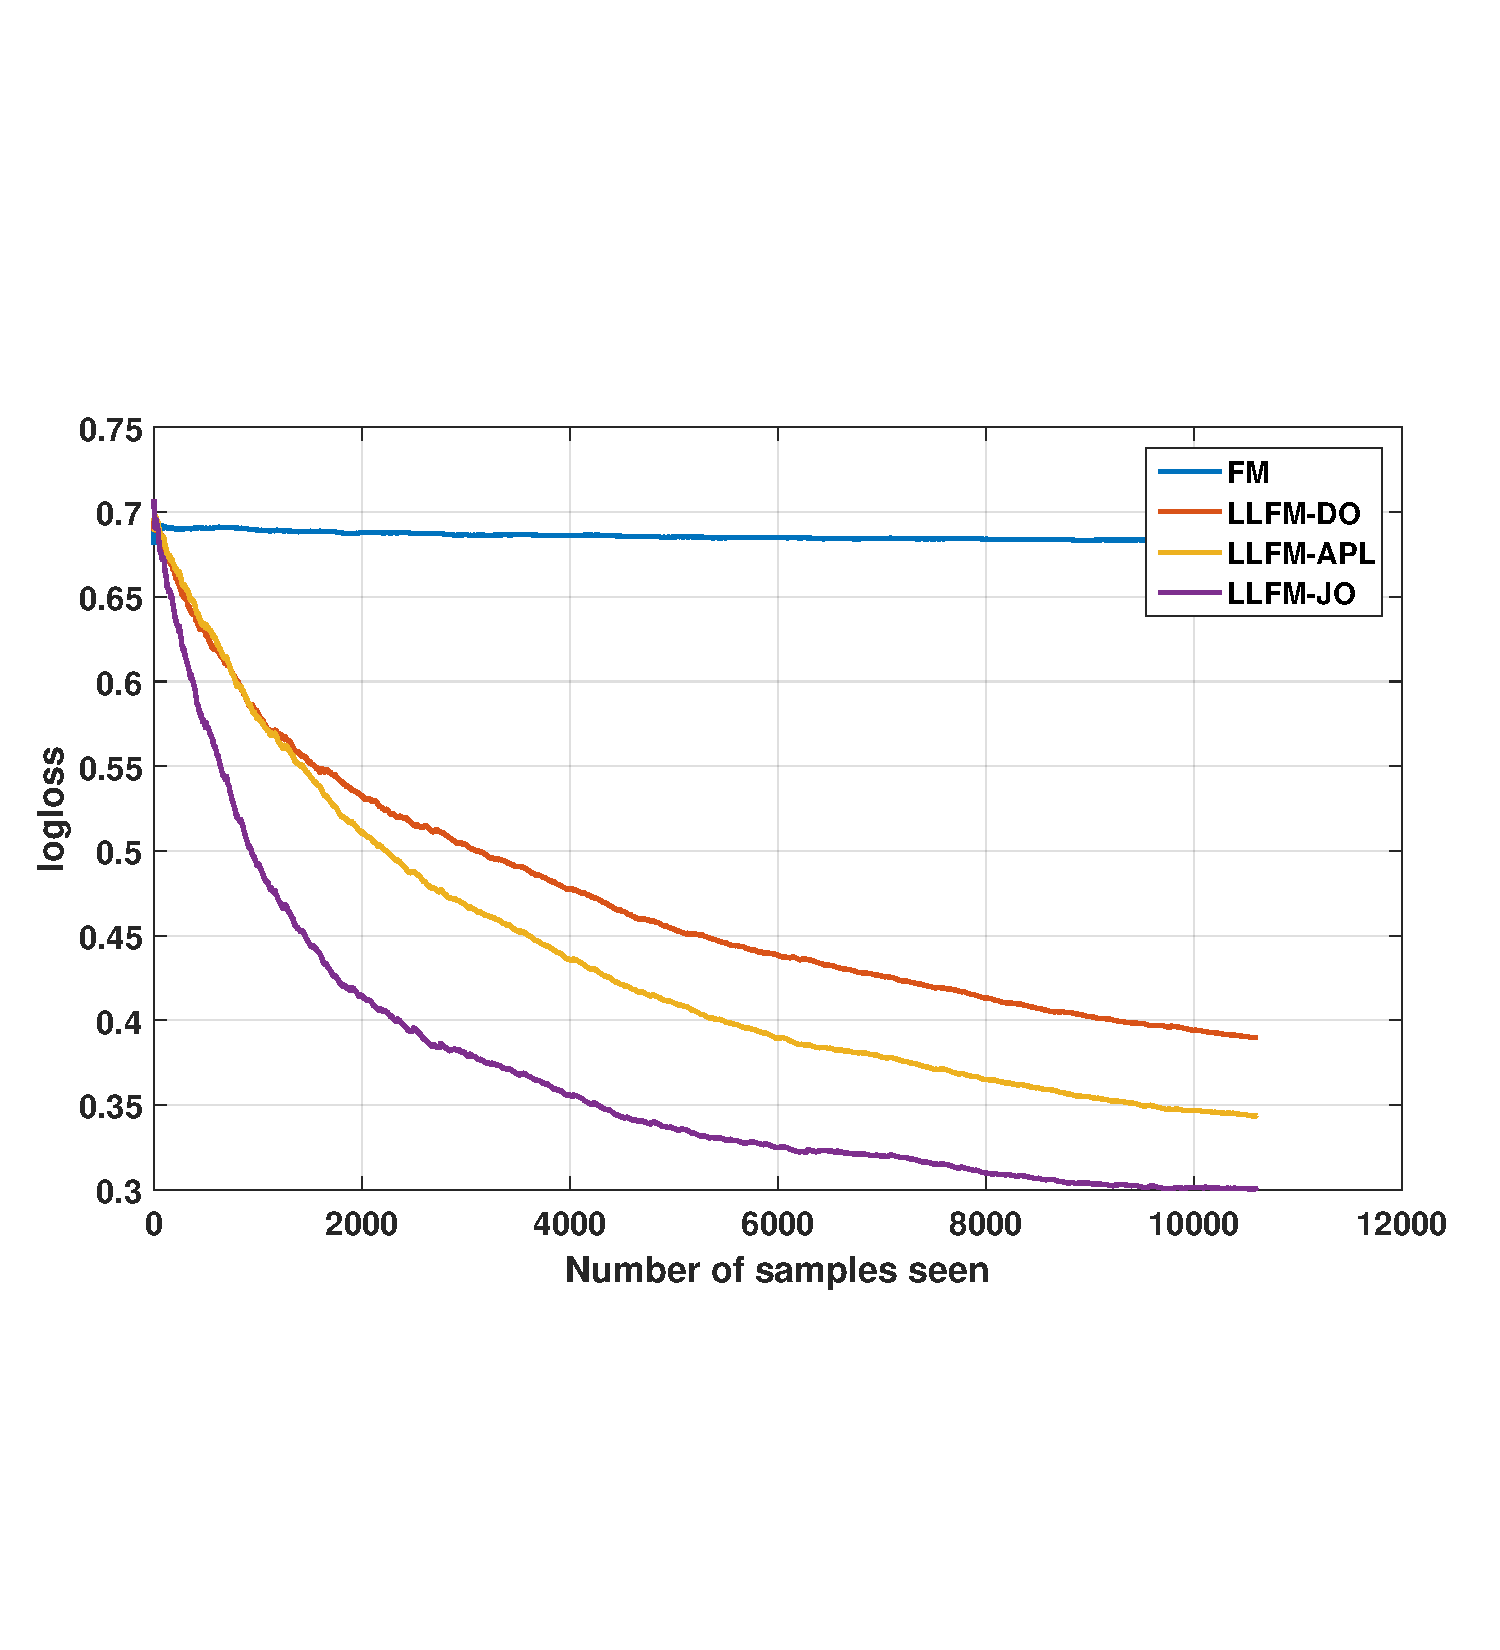
\includegraphics[width=0.5\textwidth]{Banana_learning_curve_3_sgd.pdf}
\end{figure}

\begin{figure}[!htbp]
	\centering
	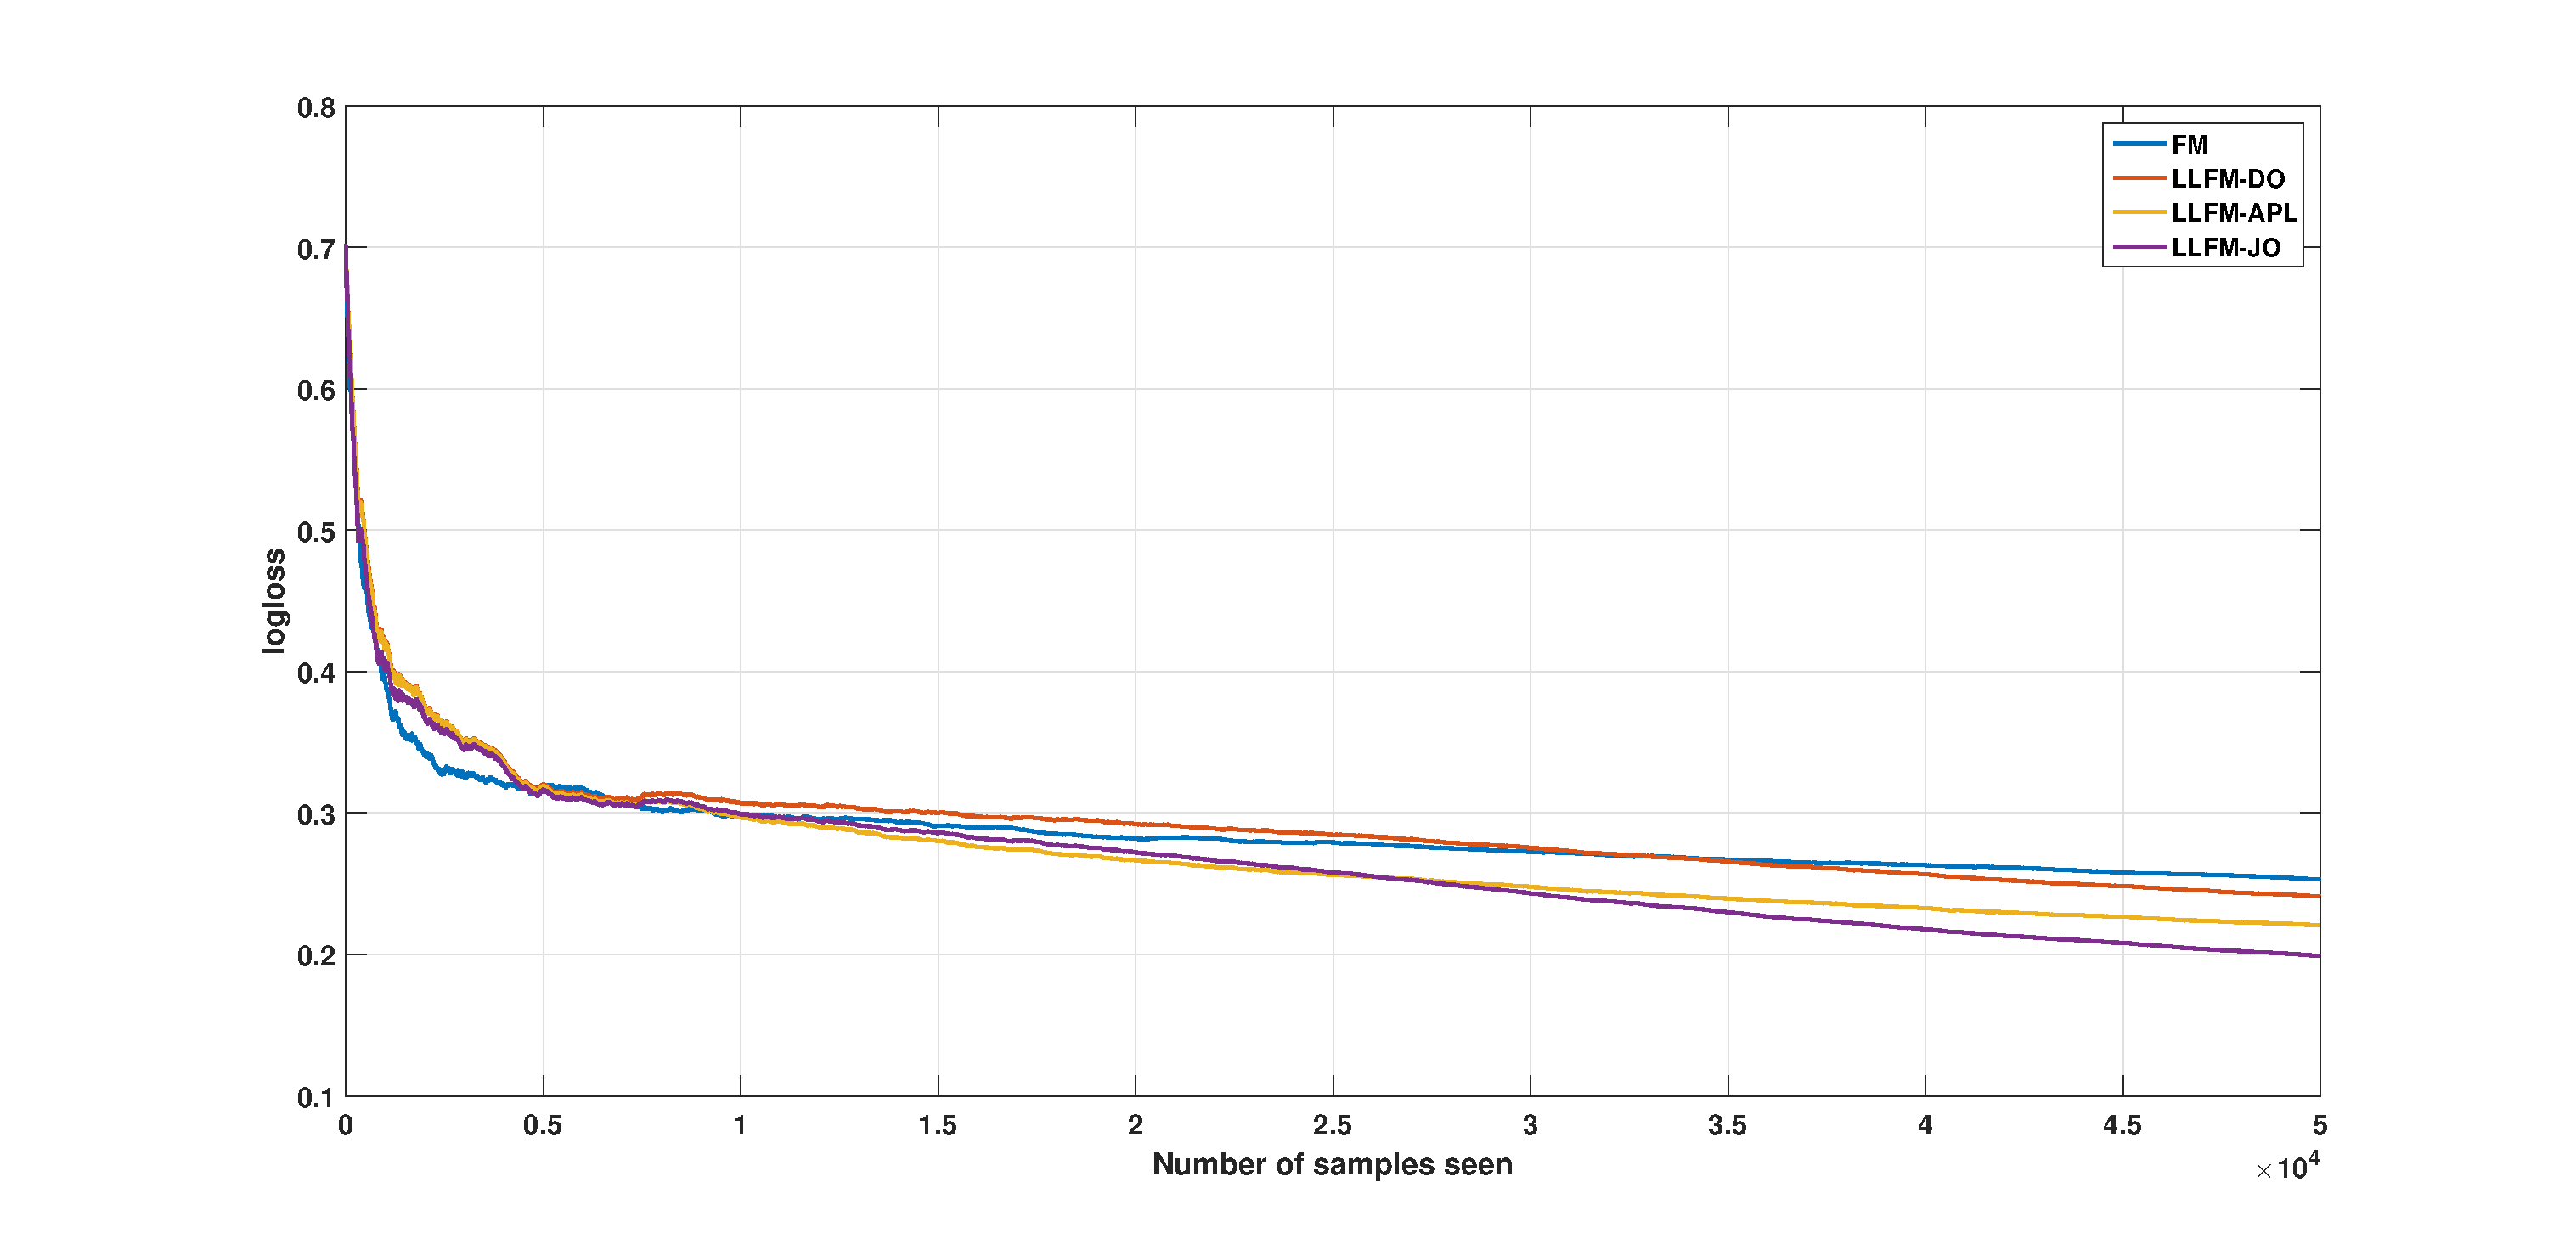
\includegraphics[width=0.5\textwidth]{IJCNN_learning_curve_1_sgd.eps}
\end{figure}
\section{Conclusion}
%% The file named.bst is a bibliography style file for BibTeX 0.99c
\bibliographystyle{named}
\bibliography{ijcai17}

\end{document}

